\begin{frame}
   \frametitle{Part 1: Capturing the Planning/Execution Tradeoff}
      \begin{tikzpicture}
      \draw[step=1,black!15,very thin,opacity=\gridopacity] (0,0) grid (12,8);
   
      % figure adapted from proposal doc
      \begin{scope}[font=\scriptsize,shift={(1.5,6.25)}]
         
         % root sets
         \node[draw,black,rounded corners,minimum height=1.5cm,minimum width=1cm]
            (Xgrasp) at (3,0) {};
         \node[above=0cm of Xgrasp] {Grasp};
         \node[draw,black,rounded corners,minimum height=1.5cm,minimum width=1cm]
            (Xdrop) at (6,0) {};
         \node[above=0cm of Xdrop] {Place};
         
         % nodes
         \node[circle,fill=black,inner sep=2] (xstart) at (0,0) {};
         \node[above=0.1cm of xstart] {$q_{\mbox{\scriptsize start}}$};
         
         % grasp choices
         \node[circle,fill=black,inner sep=2] (xg1) at (2.8,0.5) {};
         \node[circle,fill=black,inner sep=2] (xg2) at (3.1,0.1) {};
         \node[circle,fill=black,inner sep=2] (xg3) at (2.9,-0.5) {};
         % place choices
         \node[circle,fill=black,inner sep=2] (xd1) at (5.9,0.3) {};
         \node[circle,fill=black,inner sep=2] (xd2) at (6.0,-0.4) {};
         % xend 
         \node[circle,fill=black,inner sep=2] (xend) at (9,0) {};
         \node[above=0.1cm of xend] {$q_{\mbox{\scriptsize end}}$};
         
         \draw[line width=1.5mm,white]
            (xstart) .. controls (1,0.2) and (1.4,0.9) .. (xg1);
         \draw[line width=1.5mm,white]
            (xstart) .. controls (1.5,0.2) .. (xg2);
         \draw[line width=1.5mm,white]
            (xstart) .. controls (1.8,-0.6) and (1.6,-0.8) .. (xg3);
         \draw
            (xstart) .. controls (1,0.2) and (1.4,0.9) .. (xg1);
         \draw
            (xstart) .. controls (1.5,0.2) .. (xg2);
         \draw
            (xstart) .. controls (1.8,-0.6) and (1.6,-0.8) .. (xg3);
         \draw[line width=1.5mm,white]
            (xg1) -- (4.7,0.6);
         \draw
            (xg1) -- (4.7,0.6);
         \draw[line width=1.5mm,white]
            (xg2) .. controls (4.5,1) and (3.5,-1.2) .. (4.5,-0.4)
                  .. controls (5.5,0.5) and (5.0,-1.3) .. (xd2);
         \draw
            (xg2) .. controls (4.5,1) and (3.5,-1.2) .. (4.5,-0.4)
                  .. controls (5.5,0.5) and (5.0,-1.3) .. (xd2);
         \draw[line width=1.5mm,white]
            (xg3) .. controls (4.3, 0.2) and (4.5,-0.2) .. (xd1);
         \draw
            (xg3) .. controls (4.3, 0.2) and (4.5,-0.2) .. (xd1);
         % in s3
         \draw[line width=1.5mm,white]
            (xd1) .. controls (8,0.3) and (8,0.1) .. (xend);
         \draw
            (xd1) .. controls (8,0.3) and (8,0.1) .. (xend);
         
         \node[fill,black,rounded corners,minimum height=1.5cm,minimum width=1cm,
            opacity=0.1] at (3,0) {};
         \node[fill,black,rounded corners,minimum height=1.5cm,minimum width=1cm,
            opacity=0.1] at (6,0) {};
         
      \end{scope}
   
      \fill[green!20] (0.1,3.7) rectangle (11.9,4.3);
   
      \node[anchor=north] at (6,5) {\begin{minipage}{11.5cm}
         Planning for manipulation tasks poses three challenges:
         
         \begin{itemize}
         \item Challenge 1: Capturing the planning/execution tradeoff.
         \item Challenge 2: Incongruent steps impede reuse.
         \item Challenge 3: Coupled steps require long planning horizons.
         \end{itemize}
      \end{minipage}};
      
   \end{tikzpicture}
\end{frame}

%\begin{frame}
%   \begin{center}
%   \Large
%   How can we extend roadmap-based methods to reason
%   about both \emph{planning} and \emph{execution} effort?
%   \end{center}
%\end{frame}

\begin{frame}
   \frametitle{The Planning vs. Execution Tradeoff on Roadmaps}
   \begin{tikzpicture}
      \draw[step=1,black!15,very thin,opacity=\gridopacity] (0,0) grid (12,8);
      
      \node[inner sep=0] at (9,5) {%
         %{\only<1>{\includegraphics{build/talk-act1-2d,rootsonly}}}%
         {\only<1-2>{\includegraphics{build/talk-act1-2d,cfree}}}%
         %{\only<3>{\includegraphics{build/talk-act1-2d,paths}}}%
         {\only<3>{\includegraphics{build/talk-act1-2d,graph}}}%
         {\only<4->{\includegraphics{build/talk-act1-2d,astara}}}%
      };
      
      \node[draw,circle,inner sep=2pt,ultra thick,fill=red!50] at (7.05, 2.0) {};
      \node[draw,circle,inner sep=2pt,ultra thick,fill=green!50] at (7.5, 2.0) {};
      \node[anchor=west] at (7.9,2.0) {start, goal configs};
      \node[anchor=west,draw,line width=1pt,fill=blue!20,minimum width=0.75cm,minimum height=0.10cm]
         (Cfreebox) at (6.9, 1.5) {};
      \node[anchor=west] at (7.9,1.5) {$\mathcal{C}_{\mbox{\scriptsize free}}$};
      
      \only<2->{
         \node[anchor=north,fill=black!15,rounded corners] at (3,7.5)
         {\bf Focus: Roadmap methods};
      }
      
      \only<5-6>{
         \node[anchor=north,fill=blue!20,rounded corners] at (3,6.5)
         {\begin{minipage}{5.5cm}
         1. Searching roadmap graphs
         
         - survey of search methods
         
         - propose new algorithm E$^8$
         \end{minipage}};
      }
      \only<7->{
         \node[anchor=north,fill=green!20,rounded corners] at (3,6.5)
         {\begin{minipage}{5.5cm}
         1. Searching roadmap graphs
         
         - survey of search methods
         
         - propose new algorithm E$^8$
         \end{minipage}};
      }
      
      \only<6->{
         \node[anchor=north,fill=blue!20,rounded corners] at (3,4.5)
         {\begin{minipage}{5.5cm}
         2. Research questions
         
         - graphs in C-space
         \end{minipage}};
      }
   
   \end{tikzpicture}
\end{frame}

\begin{frame}
   \frametitle{Efficiency in Graph Search}
   \begin{tikzpicture}
   
      \draw[step=1,black!15,very thin,opacity=\gridopacity] (0,0) grid (12,8);
      
      % example (FIRST) problems
      \only<4-14>
      {
         \node[inner sep=0pt] at (6.5,7) {\includegraphics[width=1.5cm]{figs/rubik.png}};
         \node[inner sep=0pt,anchor=north,align=center,font=\scriptsize] at (6.5,6) {$4.3 \times 10^{19}$\\vertices};
      }
      
      \only<5-14>
      {
         \node[inner sep=0pt] at (8.5,7) {\includegraphics[width=1.5cm]{figs/15puzzle.png}};
         \node[inner sep=0pt,anchor=north,align=center,font=\scriptsize] at (8.5,6) {$2.1 \times 10^{13}$\\vertices};
      }
      
      \only<6-14>
      {
         \node[inner sep=0pt] at (10.5,7) {\includegraphics[width=1.5cm]{figs/goldberg-northwest.png}};
         \node[inner sep=0pt,anchor=north,align=center,font=\scriptsize] at (10.5,6) {1.6M\\vertices};
      }
      
      % example problems SECOND
      \only<17->
      {
         \node[inner sep=0pt] at (2.0,7) {\includegraphics[width=2.5cm]{figs/fridge-intro.png}};
         \node[inner sep=0pt,anchor=north,align=center,font=\scriptsize] at (2.0,6) {$\sim10$k\\vertices};
      }
      \only<18->
      {
         \node[inner sep=0pt] at (5.0,7) {\includegraphics[width=2.5cm]{figs/prm.png}};
         \node[inner sep=0pt,anchor=north,align=center,font=\scriptsize] at (5.0,6)
            {Motivation: PRM$^\dag$};
         % cite
         %\node[anchor=east,font=\scriptsize] at (12,0.5)
         %   {$^\dag$ Kavraki, Svestka, Latombe, Overmars, 1996.};
      }
      
      % draw graph box
      \only<1-2>{
         \node[draw,align=center,minimum height=1.3cm,anchor=south east] at (5,3.5) {
            Graph\\$G = (V,E)$\\\includegraphics[width=1cm]{build/roadmap-2d-simple}
         };
      }
      \only<3-15>{
         \node[draw,align=center,minimum height=1.3cm,anchor=south east] at (5,3.5) {
            Graph\\$G = (V,E)$\\\includegraphics[width=3cm]{build/roadmap-2d-simple}
         };
      }
      % grow using a*!
      \only<7-14>{
         \fill[white,fill opacity=0.9] (1.8,3.6) rectangle (4.9,6.7);
         \begin{scope}
            \clip (1.8,3.6) rectangle (4.9,6.7);
            \only<7>{\clip[rotate around={15:(2.0,4.8)}] (2.0,4.8) ellipse (0.5cm and 0.25cm);}
            \only<8>{\clip[rotate around={15:(2.0,4.8)}] (2.0,4.8) ellipse (1.0cm and 0.50cm);}
            \only<9>{\clip[rotate around={15:(2.0,4.8)}] (2.0,4.8) ellipse (1.4cm and 0.70cm);}
            \only<10>{\clip[rotate around={15:(2.0,4.8)}] (2.0,4.8) ellipse (1.6cm and 0.80cm);}
            \only<11>{\clip[rotate around={15:(2.0,4.8)}] (2.0,4.8) ellipse (1.9cm and 0.85cm);}
            \only<12>{\clip[rotate around={15:(2.0,4.8)}] (2.0,4.8) ellipse (2.1cm and 1.05cm);}
            \only<13-14>{\clip[rotate around={15:(2.0,4.8)}] (2.0,4.8) ellipse (2.2cm and 1.10cm);}
            \node[align=center,minimum height=1.3cm,anchor=south east] at (5,3.5) {
               \includegraphics[width=3cm]{build/roadmap-2d-simple}};
            \only<14>{\draw[rotate around={15:(2.0,4.8)},line width=4pt]
               (2.0,4.8) ellipse (2.2cm and 1.10cm);}
         \end{scope}
      }
      \only<16->{
         \node[draw,align=center,minimum height=1.3cm,anchor=south east,font=\scriptsize] at (5,3.5) {
            Graph\\$G = (V,E)$\\\includegraphics[width=0.5cm]{build/roadmap-2d-simple}
         };
      }
      
      % draw edge eval box
      \only<1-2>{
         \node[draw,align=center,anchor=south west] at (7,3.5)
            {\\Edge Weight\\$x : E \rightarrow \mathbb{R}^+$\\};
      }
      \only<3-15>{
         \begin{scope}[font=\tiny]
            \node[draw,align=center,anchor=south west] at (7,3.5)
               {\\Edge Weight\\$x : E \rightarrow \mathbb{R}^+$\\};
         \end{scope}
      }
      \only<16->{
         \node[draw,align=center,anchor=south west,inner sep=1cm] at (7,3.5)
            {\\Edge Weight\\$x : E \rightarrow \mathbb{R}^+$\\};
      }
      
      \draw[->,line width=1pt] (4,3.25) -- (4,2.75);
      \draw[->,line width=1pt] (8,3.25) -- (8,2.75);
      \node[draw,align=center,minimum height=1.0cm,minimum width=5cm,anchor=north,
         fill=blue!20,rounded corners]
         at (6,2.5) {\\$GS(G,x)$};

      % clocks
      \only<2-13>{
         % graph
         \node[fill=white,circle,inner sep=-2pt] at (5,3.5) {\LARGE%
            \only<2-6>{\showclock{0}{0}}%
            \only< 7>{\showclock{0}{10}}%
            \only< 8>{\showclock{0}{20}}%
            \only< 9>{\showclock{0}{30}}%
            \only<10>{\showclock{0}{40}}%
            \only<11>{\showclock{0}{50}}%
            \only<12>{\showclock{1}{00}}%
            \only<13>{\showclock{1}{10}}%
         };
         % edge weight
         \node[fill=white,circle,inner sep=-2pt] at (7,3.5) {\LARGE%
            \only<2-6>{\showclock{0}{0}}%
            \only< 7>{\showclock{0}{5}}%
            \only< 8>{\showclock{0}{10}}%
            \only< 9>{\showclock{0}{15}}%
            \only<10>{\showclock{0}{20}}%
            \only<11>{\showclock{0}{25}}%
            \only<12>{\showclock{0}{30}}%
            \only<13>{\showclock{0}{35}}%
         };
         % graph search
         \node[fill=white,circle,inner sep=-2pt] at (6,2.5) {\LARGE%
            \only<2-6>{\showclock{0}{0}}%
            \only< 7>{\showclock{0}{5}}%
            \only< 8>{\showclock{0}{10}}%
            \only< 9>{\showclock{0}{20}}%
            \only<10>{\showclock{0}{40}}%
            \only<11>{\showclock{1}{20}}%
            \only<12>{\showclock{2}{40}}%
            \only<13>{\showclock{5}{20}}%
         };
      }
      \only<14>{
         % graph
         \node[fill=green,circle,inner sep=-2pt] at (5,3.5) {\LARGE\showclock{1}{10}};
         % edge weight
         \node[fill=white,circle,inner sep=-2pt] at (7,3.5) {\LARGE\showclock{0}{35}};
         % graph search
         \node[fill=white,circle,inner sep=-2pt] at (6,2.5) {\LARGE\showclock{5}{20}};
      }
      \only<15-18>{
         % graph
         \node[fill=white,circle,inner sep=-2pt] at (5,3.5) {\LARGE\showclock{0}{0}};
         % edge weight
         \node[fill=white,circle,inner sep=-2pt] at (7,3.5) {\LARGE\showclock{0}{0}};
         % graph search
         \node[fill=white,circle,inner sep=-2pt] at (6,2.5) {\LARGE\showclock{0}{0}};
      }
      \only<19->{
         % graph
         \node[fill=white,circle,inner sep=-2pt] at (5,3.5) {\LARGE\showclock{0}{0}};
         % edge weight
         \node[fill=green,circle,inner sep=-2pt] at (7,3.5) {\LARGE\showclock{0}{0}};
         % graph search
         \node[fill=white,circle,inner sep=-2pt] at (6,2.5) {\LARGE\showclock{0}{0}};
      }
      
      \node[draw,align=center,shape=document] at (1.5,2) {Query\;\;\;};
      \draw[->,line width=1pt] (2.5,2) -- (3.25,2);
      \draw[->,line width=1pt] (8.75,2) -- (9.50,2);
      \node[draw,align=center,shape=document] at (10.15,2) {$\pi^*$\;\;\;};

      \only<14>{
         \node at (6,0.75) {A* is {\bf optimally efficient} w.r.t
            the number of {\bf vertices considered}.};
      }
      \only<19>{
         \node at (6,0.75) {A* is {\bf not optimally efficient} w.r.t
            the number of {\bf edges evaluated}.
         };
      }
      \only<20>{
         \node[align=center] at (6,0.75) {
            {\bf E$^4$}: \emph{Explicit graphs with Expensive Edge Evaluations}
         };
      }
      
      \only<18>{
         \node at (6,0.5) {\begin{minipage}{11.5cm}\scriptsize{
            $^\dag$\PaperPortrait\; Kavraki, Svestka, Latombe, Overmars.
               Probabilistic roadmaps for path planning in high-dimensional configuration spaces.
               IEEE Transactions on Robotics and Automation, 1996.
         }\end{minipage}};
      }
      
   \end{tikzpicture}
\end{frame}

\begin{frame}
   \frametitle{Explicit Graphs with Expensive Edge Evaluations}
   \begin{tikzpicture}
      \draw[step=1,black!15,very thin,opacity=\gridopacity] (0,0) grid (12,8);
      
      \node[inner sep=0] at (9.25,5) {%
         \includegraphics{build/talk-act1-2d,astara}%
      };
      
      % f(x) highlight
      \node[inner sep=0pt,fill=black!15,minimum height=2.8cm,minimum width=6.3cm,rounded corners]
         at (3.25,6.3) {};
      \only<2>{
         \fill[green!30] (0.1,5.85) rectangle (6.4,6.7);
         \fill[red!30] (0.1,5.0) rectangle (6.4,5.5);
      }
      
      % bfs
      \node[anchor=north west,inner sep=0pt] at (0.25,7.6) {Best-first search over paths:};
      \node[anchor=north,inner sep=0pt] at (3.25,7.0) {\begin{minipage}{6.5cm}\small{
         \algrenewcommand\algorithmicindent{0.2cm}%
         \begin{algorithmic}
         \Loop%
            \State ${\hat \pi}^* \leftarrow \argmin\limits_{\pi \in \Pi}
               \left[ \hat{f}_x(\pi) \right]$
            \State $e \leftarrow$ select from ${\hat \pi}^*$
            \State $\mbox{evaluate } x(e)$
         \EndLoop
         \end{algorithmic}
      }\end{minipage}};
      
      \only<3>{
         % fx(pi) execution path cost
         \node[anchor=north,inner sep=0pt] at (3.25,5.1) {\begin{minipage}{6cm}\small{
            \begin{equation*}
               \arraycolsep=1.4pt
               \hat{f}_x(\pi) = \sum_{e \in \pi} \left\{
               \begin{array}{cl}
                  x(e) & \mbox{if edge } e \mbox{ evaluated}  \\
                  \hat{x}(e) & \mbox{otherwise} \\
               \end{array}
               \right.
            \end{equation*}
         }\end{minipage}};
         
         % ensemble highlight
         \node[anchor=north,shape=document,draw,inner sep=0.25cm] at (6,2.25) {\begin{minipage}{8.5cm}\small{
            Effort model:
            
            $x(e)$ : edge evaluation function \emph{(expensive to compute)}
            
            ${\hat x}(e)$ : optimistic estimate of value of $x(e)$
         }\end{minipage}};
      }
      
      \only<1-2>{
         \node at (6,0.5) {\begin{minipage}{11.5cm}\scriptsize{
            \PaperPortrait\; Bohlin, Kavraki.
            ``Path planning using Lazy PRM,'' ICRA, 2000.
         }\end{minipage}};
      }
      
      %\only<2>{
      %   \node[fill=white,opacity=0.9] at (9.25,3) {This is Lazy PRM! Animate!};
      %}
   
   \end{tikzpicture}
\end{frame}

\begin{frame}
   \frametitle{Survey of Graph Search Algorithms}
   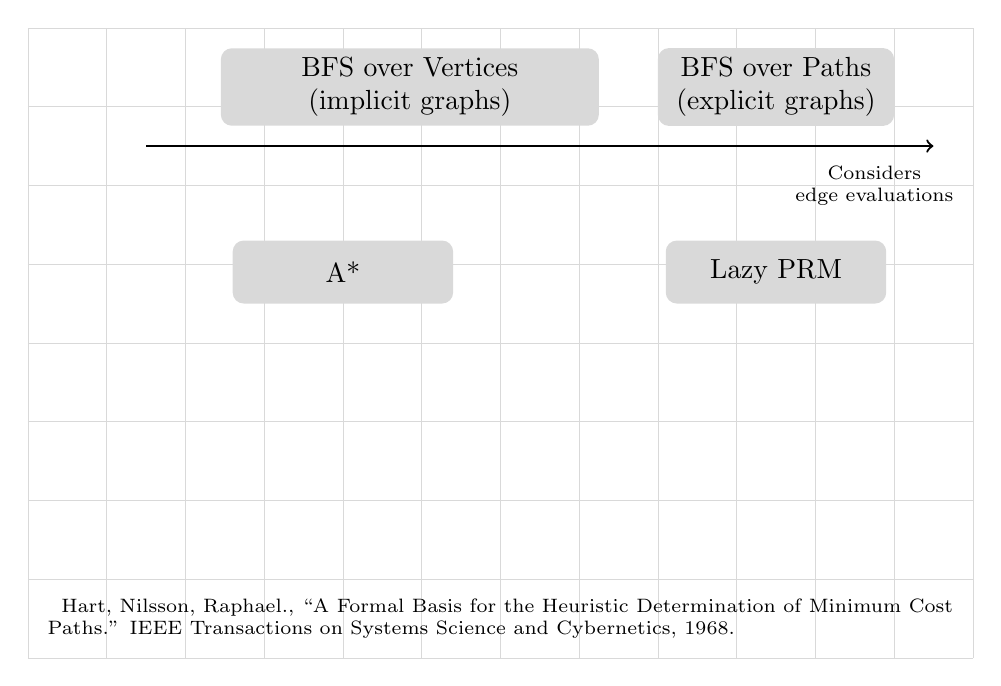
\begin{tikzpicture}
      \draw[step=1,black!15,very thin,opacity=\gridopacity] (0,0) grid (12,8);
      
      \node[align=center,fill=black!15,minimum width=4.8cm,rounded corners]
         at (4.85,7.25) {BFS over Vertices\\(implicit graphs)};
      \node[align=center,fill=black!15,minimum width=3cm,rounded corners]
         at (9.5,7.25) {BFS over Paths\\(explicit graphs)};
      
      %\draw[dashed] (7.5,7.75) -- (7.5,1.25);
      %\draw[dashed,->] (7.5,1.5) -- (8.5,1.5);
      %\node[align=center,font=\scriptsize]
      %   at (9.5,1.5) {Expressiveness\\of objective};

      % x axis
      \draw[->,thick] (1.5,6.5) -- (11.5,6.5);
      \node[align=center,font=\scriptsize]
         at (10.75,6) {Considers\\edge evaluations};
      
      %\node[font=\small] at (1,7) {Heuristics:};
      
      % y axis
      %\draw[->,thick] (2.2,7) -- (2.2,2);
      %\node[align=center,font=\scriptsize]
      %   at (2.2,1.5) {Expressiveness\\of heuristics};

      %\node[align=center,fill=black!15,rounded corners,minimum width=1.8cm,minimum height=0.4cm]
      %   at (1,5.9) {none};
      %\node[fill=black!15,rounded corners,minimum height=0.8cm,minimum width=2.8cm]
      %   at (4,5.9) {Dijkstra's};

      %\node[align=center,fill=black!15,rounded corners,minimum width=1.8cm,minimum height=0.4cm]
      %   at (1,4.9) {${\hat x}$};
      \node[fill=black!15,rounded corners,minimum height=0.8cm,minimum width=2.8cm]
         at (4,4.9) {A*};
      %\node[fill=black!15,rounded corners,minimum height=0.8cm,font=\scriptsize,align=center]
      %   at (6.5,4.9) {(E)PEA*\\OGA*};
      \node[fill=black!15,rounded corners,minimum height=0.8cm,minimum width=2.8cm]
         at (9.5,4.9) {Lazy PRM};
      
      %\node[align=center,fill=black!15,rounded corners,minimum width=1.8cm,minimum height=0.4cm]
      %   at (1,3.9) {${\hat x}, {\hat p} \propto {\hat x}$};
      %\node[fill=black!15,rounded corners,minimum height=0.8cm,minimum width=2.8cm]
      %   at (4,3.9) {Weighted A*};
      
      %\node[align=center,fill=black!15,rounded corners,minimum width=1.8cm,minimum height=0.4cm]
      %   at (1,2.9) {${\hat x}, {\hat p}$};
      %\node[fill=black!15,rounded corners,minimum height=0.8cm,minimum width=2.8cm]
      %   at (4,2.9) {BUGSY};
      %\node[fill=blue!20,rounded corners,minimum height=0.8cm,minimum width=2.8cm]
      %   at (9.5,2.9) {E$^8$};
      
      
      \only<1>{
         \node at (6,0.5) {\begin{minipage}{11.5cm}\scriptsize{
            \PaperPortrait\; Hart, Nilsson, Raphael.,
            ``A Formal Basis for the Heuristic Determination of Minimum Cost Paths.''
            IEEE Transactions on Systems Science and Cybernetics, 1968.
         }\end{minipage}};
      }
      
      
   \end{tikzpicture}
\end{frame}

\begin{frame}
   \frametitle{Advantages of Best-First Search over Paths}
   
   Advantages of BFS over Paths (e.g. the Lazy PRM):
   \begin{itemize}
   \item<2-> Naturally minimizes number of evaluated edges
   \item<3-> Allows for more flexible path evaluation strategies
   \begin{center}
      \begin{tikzpicture}
         \draw[step=1,black!15,very thin,opacity=0] (0,0) grid (8,2);
         
         \only<28>{\node[inner sep=0pt,rounded corners,fill=blue!20,
            minimum width=2.7cm,minimum height=1.7cm] at (1.5,1) {};}
         \only<4>\fill[black!50] (0.5,0.5) circle (0.25cm);
         \only<6>\fill[black!50] (1.5,0.5) circle (0.25cm);
         \only<8>\fill[black!50] (2.5,0.5) circle (0.25cm);
         \only<10>\draw[black!50,line width=5pt] (0.5,0.5) -- (2.5,0.5);
         \draw[dashed]
            (1.5,0.5) -- (1.5,1.5) -- (0.5,1.5) -- (0.5,0.5) -- (2.5,0.5)
            -- (2.5,1.5) -- (1.5,1.5);
         \only<5-8>{\draw[very thick] (0.5,1.5) -- (0.5,0.5) -- (1.5,0.5);}
         \only<7-8>{\draw[very thick] (1.5,1.5) -- (1.5,0.5) -- (2.5,0.5);}
         \only<11->{\draw[very thick] (0.5,0.5) -- (2.5,0.5);}
         \node[draw,circle,inner sep=2pt,ultra thick,fill=red!50] at (0.5,0.5) {};
         \node[draw,circle,inner sep=2pt,ultra thick,fill=green!50] at (2.5,0.5) {};
         \fill[black]
            (0.5,1.5) circle (0.07cm)
            (1.5,0.5) circle (0.07cm)
            (1.5,1.5) circle (0.07cm)
            (2.5,1.5) circle (0.07cm);
         
         \only<22>\draw[black!50,line width=5pt] (4.5,0.5) -- (7.5,0.5);
         \only<24>\draw[black!50,line width=5pt]
            (4.5,0.5) -- (5.5,1.5) -- (6.5,1.5) -- (7.5,0.5);
         \fill[black] (5.9,0.0) rectangle (6.1,0.9);
         \draw[dashed] (4.5,0.5) -- (7.5,0.5) -- (6.5,1.5) -- (5.5,1.5) -- (4.5,0.5);
         \only<13-20>{\draw[very thick] (5.5,1.5) -- (4.5,0.5) -- (5.5,0.5);}
         \only<15-20,23->{\draw[very thick,red] (5.5,0.5) -- (6.5,0.5);}
         \only<17-20>{\draw[very thick] (5.5,1.5) -- (6.5,1.5);}
         \only<19-20>{\draw[very thick] (6.5,1.5) -- (7.5,0.5);}
         \only<25->\draw[very thick]
            (4.5,0.5) -- (5.5,1.5) -- (6.5,1.5) -- (7.5,0.5);
         \node[draw,circle,inner sep=2pt,ultra thick,fill=red!50] at (4.5,0.5) {};
         \node[draw,circle,inner sep=2pt,ultra thick,fill=green!50] at (7.5,0.5) {};
         \fill[black]
            (5.5,0.5) circle (0.07cm)
            (6.5,0.5) circle (0.07cm)
            (5.5,1.5) circle (0.07cm)
            (6.5,1.5) circle (0.07cm);
         \only<12>\fill[black!50] (4.5,0.5) circle (0.25cm);
         \only<14>\fill[black!50] (5.5,0.5) circle (0.25cm);
         \only<16>\fill[black!50] (5.5,1.5) circle (0.25cm);
         \only<18>\fill[black!50] (6.5,1.5) circle (0.25cm);
         \only<20>\fill[black!50] (7.5,0.5) circle (0.25cm);
         
      \end{tikzpicture}
   \end{center}
   \item<26-> Admits more natural expression of our path objective
   \begin{center}
      \begin{tikzpicture}
         \node[anchor=west,inner xsep=0pt,fill=black!15,minimum height=2cm,rounded corners]
            at (0,6.75) {\begin{minipage}{3.25cm}\small{
            \algrenewcommand\algorithmicindent{0.0cm}%
            \algrenewcommand\algorithmicloop{\!\!\!\!\textbf{loop}}
            \begin{algorithmic}
            \Loop%
               \State $\pi^* \leftarrow \argmin\limits_{\pi \in \Pi} f(\pi)$
               \State \textsc{EvalPath}$(\pi^*)$
            \EndLoop
            \end{algorithmic}
         }\end{minipage}};
      \end{tikzpicture}
   \end{center}
   \item<27-> Extends naturally to multi-query regime
   \end{itemize}
   
\end{frame}

\begin{frame}
   \frametitle{Survey of Graph Search Algorithms}
   \begin{tikzpicture}
      \draw[step=1,black!15,very thin,opacity=\gridopacity] (0,0) grid (12,8);
      
      \node[align=center,fill=black!15,minimum width=4.8cm,rounded corners]
         at (4.85,7.25) {BFS over Vertices\\(implicit graphs)};
      \node[align=center,fill=black!15,minimum width=3cm,rounded corners]
         at (9.5,7.25) {BFS over Paths\\(explicit graphs)};
      
      \only<3>{
         \draw[dashed] (7.6,7.75) -- (7.6,1.25);
         \draw[dashed,->] (7.6,1.5) -- (8.5,1.5);
         \node[align=center,font=\scriptsize]
            at (9.7,1.9) {Flexibility of\\evaluation order};
         \node[align=center,font=\scriptsize]
            at (9.7,1.1) {Expressiveness\\of objective};
      }

      % x axis
      \draw[->,thick] (1.5,6.5) -- (11.5,6.5);
      \node[align=center,font=\scriptsize]
         at (10.75,6) {Considers\\edge evaluations};
      
      %\node[font=\small] at (1,7) {Heuristics:};
      
      % y axis
      %\draw[->,thick] (2.2,7) -- (2.2,2);
      %\node[align=center,font=\scriptsize]
      %   at (2.2,1.5) {Expressiveness\\of heuristics};

      %\node[align=center,fill=black!15,rounded corners,minimum width=1.8cm,minimum height=0.4cm]
      %   at (1,5.9) {none};
      %\node[fill=black!15,rounded corners,minimum height=0.8cm,minimum width=2.8cm]
      %   at (4,5.9) {Dijkstra's};

      %\node[align=center,fill=black!15,rounded corners,minimum width=1.8cm,minimum height=0.4cm]
      %   at (1,4.9) {${\hat x}$};
      \node[fill=black!15,rounded corners,minimum height=0.8cm,minimum width=2.8cm]
         at (4,4.9) {A*};
      \only<2>{\node[fill=blue!20,rounded corners,minimum height=0.8cm,font=\scriptsize,align=center]
         at (6.5,4.9) {(E)PEA*\\OGA*};}
      \only<3>{\node[fill=black!15,rounded corners,minimum height=0.8cm,font=\scriptsize,align=center]
         at (6.5,4.9) {(E)PEA*\\OGA*};}
      \node[fill=black!15,rounded corners,minimum height=0.8cm,minimum width=2.8cm]
         at (9.5,4.9) {Lazy PRM};
      
      %\node[align=center,fill=black!15,rounded corners,minimum width=1.8cm,minimum height=0.4cm]
      %   at (1,3.9) {${\hat x}, {\hat p} \propto {\hat x}$};
      %\node[fill=black!15,rounded corners,minimum height=0.8cm,minimum width=2.8cm]
      %   at (4,3.9) {Weighted A*};
      
      %\node[align=center,fill=black!15,rounded corners,minimum width=1.8cm,minimum height=0.4cm]
      %   at (1,2.9) {${\hat x}, {\hat p}$};
      %\node[fill=black!15,rounded corners,minimum height=0.8cm,minimum width=2.8cm]
      %   at (4,2.9) {BUGSY};
      %\node[fill=blue!20,rounded corners,minimum height=0.8cm,minimum width=2.8cm]
      %   at (9.5,2.9) {E$^8$};
      
      \only<2>{
      
      
         \node at (6,2.1) {\begin{minipage}{11.5cm}\scriptsize{
            \PaperPortrait\; Yoshizumi, Teruhisa Miura, Toru Ishida.
            ``A* with Partial Expansion for Large Branching Factor Problems.'' AAAI 2000.
         }\end{minipage}};
      
         \node at (6,1.3) {\begin{minipage}{11.5cm}\scriptsize{
            \PaperPortrait\; Felner, Goldenberg, Sharon, Stern, Beja, Sturtevant, Schaeffer, Holte.
            ``Partial-Expansion A* with Selective Node Generation.'' AAAI 2012.
         }\end{minipage}};
         
         \node at (6,0.5) {\begin{minipage}{11.5cm}\scriptsize{
            \PaperPortrait\;  Goldenberg, Felner, Sturtevant, Holte, Schaeffer.
            ``Optimal-Generation Variants of EPEA*''. SOCS 2013.
         }\end{minipage}};
         
        
         
      }
      
   \end{tikzpicture}
\end{frame}

\begin{frame}
   \frametitle{Challenge 1: The Planning/Execution Tradeoff}
   \begin{tikzpicture}
   
      \draw[step=1,black!15,very thin,opacity=\gridopacity] (0,0) grid (12,8);
      
      \node[inner sep=0pt] at (3.5,5.5) {\includegraphics[width=4cm]{figs/fridge-intro.png}};
      \node[inner sep=0pt,anchor=north] at (3.5,4.0)
         {\begin{minipage}{4cm}\centering
            Autonomous maniptulation tasks
            
            (plan then execute)
         \end{minipage}};
      
      \node[inner sep=0pt] at (8.5,5.0) {\includegraphics{build/ensemble-effort-plot-1}};
      
      %\only<2->
      %{
      %   \node[fill=blue!20,rounded corners,align=center] at (6,1.5)
      %   {
      %   Key Insight: Optimize for combined\\
      %   planning \& execution effort \emph{explicitly}!
      %   };
      %}
         
   \end{tikzpicture}
\end{frame}

\begin{frame}
   \frametitle{Survey of Graph Search Algorithms}
   \begin{tikzpicture}
      \draw[step=1,black!15,very thin,opacity=\gridopacity] (0,0) grid (12,8);
      
      \node[align=center,fill=black!15,minimum width=4.8cm,rounded corners]
         at (4.85,7.25) {BFS over Vertices\\(implicit graphs)};
      \node[align=center,fill=black!15,minimum width=3cm,rounded corners]
         at (9.5,7.25) {BFS over Paths\\(explicit graphs)};
      
      \draw[dashed] (7.6,7.75) -- (7.6,1.25);
      \draw[dashed,->] (7.6,1.5) -- (8.5,1.5);
      \node[align=center,font=\scriptsize]
         at (9.7,1.9) {Flexibility of\\evaluation order};
      \node[align=center,font=\scriptsize]
         at (9.7,1.1) {Expressiveness\\of objective};

      % x axis
      \draw[->,thick] (1.5,6.5) -- (11.5,6.5);
      \node[align=center,font=\scriptsize]
         at (10.75,6) {Considers\\edge evaluations};
      
      \only<2->{\node[font=\small] at (1,7) {Heuristics:};}
      
      % y axis
      \only<2-4>{\draw[thick] (2.2,7) -- (2.2,2);}
      \only<5->{ 
         \draw[->,thick] (2.2,7) -- (2.2,2);
         \node[align=center,font=\scriptsize]
            at (2.2,1.5) {Expressiveness\\of heuristics};
      }

      \only<4->{
         \node[align=center,fill=black!15,rounded corners,minimum width=1.8cm,minimum height=0.4cm]
            at (1,5.9) {none};
         \node[fill=black!15,rounded corners,minimum height=0.8cm,minimum width=2.8cm]
            at (4,5.9) {Dijkstra's};
      }

      \only<3->{
         \node[align=center,fill=black!15,rounded corners,minimum width=1.8cm,minimum height=0.4cm]
         at (1,4.9) {${\hat x}$};
      }
      \node[fill=black!15,rounded corners,minimum height=0.8cm,minimum width=2.8cm]
         at (4,4.9) {A*};
      \node[fill=black!15,rounded corners,minimum height=0.8cm,font=\scriptsize,align=center]
         at (6.5,4.9) {(E)PEA*\\OGA*};
      \node[fill=black!15,rounded corners,minimum height=0.8cm,minimum width=2.8cm]
         at (9.5,4.9) {Lazy PRM};
      
      %\node[align=center,fill=black!15,rounded corners,minimum width=1.8cm,minimum height=0.4cm]
      %   at (1,3.9) {${\hat x}, {\hat p} \propto {\hat x}$};
      %\node[fill=black!15,rounded corners,minimum height=0.8cm,minimum width=2.8cm]
      %   at (4,3.9) {Weighted A*};
      
      \only<6->{
         \node[align=center,fill=black!15,rounded corners,minimum width=1.8cm,minimum height=0.4cm]
            at (1,2.9) {${\hat x}, {\hat p}$};
      }
      \only<7->{
         \node[fill=black!15,rounded corners,minimum height=0.8cm,minimum width=2.8cm]
            at (4,2.9) {BUGSY$^\dag$};
      }
      %\node[fill=blue!20,rounded corners,minimum height=0.8cm,minimum width=2.8cm]
      %   at (9.5,2.9) {E$^8$};
      
      \only<8->{
         \draw[->,thick] (9.5,4.25) -- (9.5,3.5);
      };
      \only<9->{
         \draw[->,thick] (5.5,2.9) -- (9,2.9);
      };
      \only<10->{
         \node[] at (9.5,2.9) {\large ?};
      };
      
      \only<7->{
         \node at (5,0.5) {\begin{minipage}{9cm}\scriptsize{
            $^\dag$\PaperPortrait\; W. Ruml and M. B. Do. Best-first Utility-Guided Search.\\
            International Joint Conference on Artificial Intelligence, 2007.
         }\end{minipage}};
      }
      
   \end{tikzpicture}
\end{frame}

\begin{frame}
   \frametitle{Explicit Graphs with Expensive Edge Evaluations}
   \begin{tikzpicture}
   
      \draw[step=1,black!15,very thin,opacity=\gridopacity] (0,0) grid (12,8);
      
      \node[inner sep=0] at (9.25,5) {%
         \includegraphics{build/talk-act1-2d,astara}%
      };
      
      % f(x) highlight
      \node[inner sep=0pt,fill=black!15,minimum height=2.8cm,minimum width=6.3cm,rounded corners]
         at (3.25,6.3) {};
      \only<4-6>{\fill[green!30] (2.65,5.9) rectangle (6.4,6.7);}
      
      % bfs
      \node[anchor=north west,inner sep=0pt] at (0.25,7.6) {Best-first search over paths:};
      \node[anchor=north,inner sep=0pt] at (3.25,7.0) {\begin{minipage}{6.5cm}\small{
         \algrenewcommand\algorithmicindent{0.2cm}%
         \begin{algorithmic}
         \Loop%
            \only<1-3>{
               \State ${\hat \pi}^* \leftarrow \argmin\limits_{\pi \in \Pi}
                  \left[ \hat{f}_x(\pi) \right]$
            }
            \only<4-6>{
               \State ${\hat \pi}^* \leftarrow \argmin\limits_{\pi \in \Pi}
                  \left[ (1-\lambda) \hat{f}_x(\pi) + \lambda \hat{f}_p(\pi) \right]$
            }
            \State $e \leftarrow$ select from ${\hat \pi}^*$
            \State $\mbox{evaluate } x(e)$
         \EndLoop
         \end{algorithmic}
      }\end{minipage}};
      
      % fx(pi) execution path cost
      \node[anchor=north,inner sep=0pt] at (3.25,5.1) {\begin{minipage}{6cm}\small{
         \begin{equation*}
            \arraycolsep=1.4pt
            \hat{f}_x(\pi) = \sum_{e \in \pi} \left\{
            \begin{array}{cl}
               x(e) & \mbox{if edge } e \mbox{ evaluated}  \\
               \hat{x}(e) & \mbox{otherwise} \\
            \end{array}
            \right.
         \end{equation*}
      }\end{minipage}};
      
      % fp(pi) execution path cost
      \only<3-6>{
      \fill[green!30] (0.1,2.5) rectangle (6.4,3.6);
      \node[anchor=north,inner sep=0pt] at (3.25,3.9) {\begin{minipage}{6cm}\small{
         \begin{equation*}
            \arraycolsep=1.4pt
            \hat{f}_p(\pi) = \sum_{e \in \pi} \left\{
            \begin{array}{cl}
               0 & \mbox{if edge } e \mbox{ evaluated}  \\
               \hat{p}(e) & \mbox{otherwise} \\
            \end{array}
            \right.
         \end{equation*}
      }\end{minipage}};
      }
      
      % p(e) highlight
      \only<2-6>{\fill[green!30] (1.5,0.3) rectangle (10.5,0.8);}
      % ensemble highlight
      \only<6>{\fill[green!30] (1.6,1.6) rectangle (5.3,2.1);}
      \node[anchor=north,shape=document,draw,inner sep=0.25cm] at (6,2.25) {\begin{minipage}{8.5cm}\small{
         \only<1-5>{Effort model:}
         \only<6>{\emph{Ensemble Effort} model:}
         
         $x(e)$ : edge evaluation function \emph{(expensive to compute)}
         
         ${\hat x}(e)$ : optimistic estimate of value of $x(e)$
         
         \only<2-6>{
            ${\hat p}(e)$ : optimistic estimate of \emph{evaluating} $x(e)$
         }
         
      }\end{minipage}};
      
      %\only<5-6>{
      %   \node[fill=white,opacity=0.9] at (9.25,3) {Animate example!};
      %}
   
   \end{tikzpicture}
\end{frame}

\begin{frame}
   \frametitle{The E$^8$ Algorithm}
   \begin{tikzpicture}
   
      \draw[step=1,black!15,very thin,opacity=\gridopacity] (0,0) grid (12,8);
      
      \node[anchor=north,shape=document,draw,inner sep=0.25cm] at (6,7.75) {\begin{minipage}{8.5cm}\small{
         Ensemble Effort model:
         
         $x(e)$ : execution effort function \emph{(expensive to compute)}
         
         ${\hat x}(e)$ : optimistic estimate of execution effort for edge $e$
         
         ${\hat p}(e)$ : optimistic estimate of planning effort for edge $e$
      }\end{minipage}};
      
      \draw[->,line width=1pt] (6,5.5) -- (6,5.0);
      
      % alg
      \node[anchor=west,inner xsep=0pt,fill=black!15,minimum height=2cm,rounded corners]
      at (0,3.75) {\begin{minipage}{3.25cm}\small{
         \algrenewcommand\algorithmicindent{0.0cm}%
         \algrenewcommand\algorithmicloop{\!\!\!\!\textbf{loop}}
         \begin{algorithmic}
         \Loop%
            \State $\pi^* \leftarrow \argmin\limits_{\pi \in \Pi} \hat{f}(\pi)$
            \State \textsc{EvalPath}$(\pi^*)$
         \EndLoop
         \end{algorithmic}
      }\end{minipage}};
      
      % f(pi) execution path cost
      \node[anchor=west,inner xsep=0pt,fill=black!15,minimum height=2cm,rounded corners]
      at (3.5,3.75) {\begin{minipage}{8.5cm}\small{%
         \vspace{-0.3cm}
         \begin{equation*}%
            \arraycolsep=1.4pt
            \hat{f}(\pi) = \sum_{e \in \pi} \left\{
            \begin{array}{cl}
               (1-\lambda) x(e) & \mbox{if edge } e \mbox{ evaluated} \\
               (1-\lambda) \hat{x}(e) + \lambda \hat{p}(e) & \mbox{otherwise} \\
            \end{array}
            \right.
         \end{equation*}
      }\end{minipage}};
      
      \node[inner sep=0pt] at (6,1.5) {\begin{minipage}{12cm}\centering
         \emph{Exploiting Ensemble Effort Estimates\\
         on Explicit graphs\\
         with Expensive Edge Evaluations}
      \end{minipage}};
   
   \end{tikzpicture}
\end{frame}

\begin{frame}
   \frametitle{Survey of Graph Search Algorithms}
   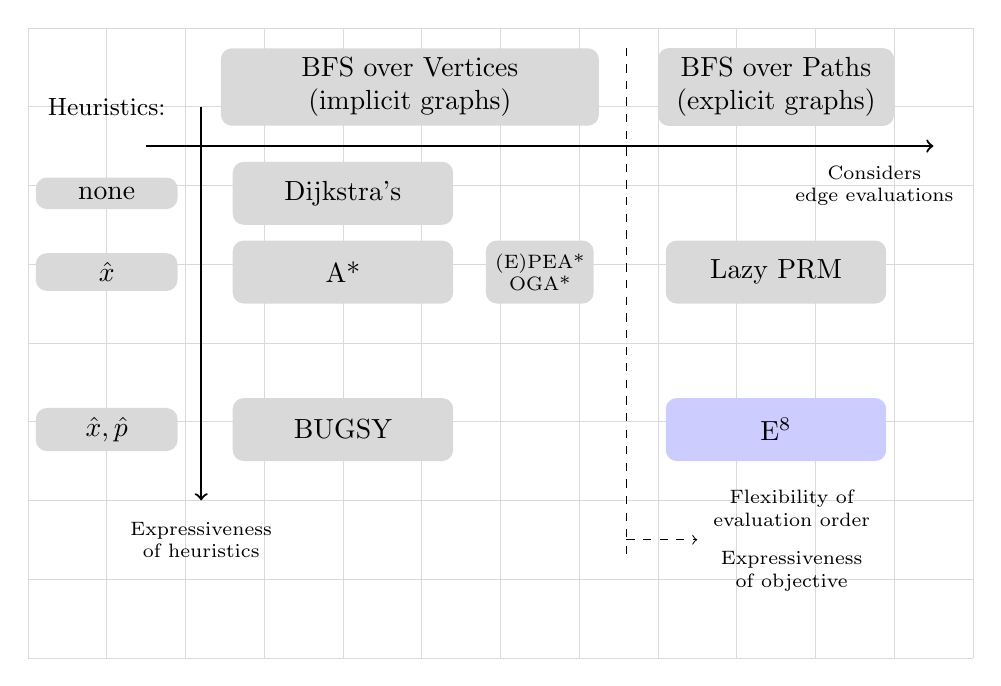
\begin{tikzpicture}
      \draw[step=1,black!15,very thin,opacity=\gridopacity] (0,0) grid (12,8);
      
      \node[align=center,fill=black!15,minimum width=4.8cm,rounded corners]
         at (4.85,7.25) {BFS over Vertices\\(implicit graphs)};
      \node[align=center,fill=black!15,minimum width=3cm,rounded corners]
         at (9.5,7.25) {BFS over Paths\\(explicit graphs)};
      
      \draw[dashed] (7.6,7.75) -- (7.6,1.25);
      \draw[dashed,->] (7.6,1.5) -- (8.5,1.5);
      \node[align=center,font=\scriptsize]
         at (9.7,1.9) {Flexibility of\\evaluation order};
      \node[align=center,font=\scriptsize]
         at (9.7,1.1) {Expressiveness\\of objective};

      % x axis
      \draw[->,thick] (1.5,6.5) -- (11.5,6.5);
      \node[align=center,font=\scriptsize]
         at (10.75,6) {Considers\\edge evaluations};
      
      \node[font=\small] at (1,7) {Heuristics:};
      
      % y axis
      \draw[->,thick] (2.2,7) -- (2.2,2);
      \node[align=center,font=\scriptsize]
         at (2.2,1.5) {Expressiveness\\of heuristics};

      \node[align=center,fill=black!15,rounded corners,minimum width=1.8cm,minimum height=0.4cm]
         at (1,5.9) {none};
      \node[fill=black!15,rounded corners,minimum height=0.8cm,minimum width=2.8cm]
         at (4,5.9) {Dijkstra's};

      \node[align=center,fill=black!15,rounded corners,minimum width=1.8cm,minimum height=0.4cm]
         at (1,4.9) {${\hat x}$};
      \node[fill=black!15,rounded corners,minimum height=0.8cm,minimum width=2.8cm]
         at (4,4.9) {A*};
      \node[fill=black!15,rounded corners,minimum height=0.8cm,font=\scriptsize,align=center]
         at (6.5,4.9) {(E)PEA*\\OGA*};
      \node[fill=black!15,rounded corners,minimum height=0.8cm,minimum width=2.8cm]
         at (9.5,4.9) {Lazy PRM};
      
      %\node[align=center,fill=black!15,rounded corners,minimum width=1.8cm,minimum height=0.4cm]
      %   at (1,3.9) {${\hat x}, {\hat p} \propto {\hat x}$};
      %\node[fill=black!15,rounded corners,minimum height=0.8cm,minimum width=2.8cm]
      %   at (4,3.9) {Weighted A*};
      
      \node[align=center,fill=black!15,rounded corners,minimum width=1.8cm,minimum height=0.4cm]
         at (1,2.9) {${\hat x}, {\hat p}$};
      \node[fill=black!15,rounded corners,minimum height=0.8cm,minimum width=2.8cm]
         at (4,2.9) {BUGSY};
      \only<2>{
         \node[fill=blue!20,rounded corners,minimum height=0.8cm,minimum width=2.8cm]
            at (9.5,2.9) {E$^8$};
      }
      
   \end{tikzpicture}
\end{frame}

\begin{frame}
   \frametitle{Simplification with Proportional Heuristics}
   \begin{tikzpicture}
   
      \draw[step=1,black!15,very thin,opacity=\gridopacity] (0,0) grid (12,8);
      
      % alg
      \node[anchor=west,inner xsep=0pt,fill=black!15,minimum height=2cm,rounded corners]
      at (0,6.75) {\begin{minipage}{3.25cm}\small{
         \algrenewcommand\algorithmicindent{0.0cm}%
         \algrenewcommand\algorithmicloop{\!\!\!\!\textbf{loop}}
         \begin{algorithmic}
         \Loop%
            \State $\pi^* \leftarrow \argmin\limits_{\pi \in \Pi} \hat{f}(\pi)$
            \State \textsc{EvalPath}$(\pi^*)$
         \EndLoop
         \end{algorithmic}
      }\end{minipage}};
      
      % f(pi) execution path cost
      \node[anchor=west,inner xsep=0pt,fill=black!15,minimum height=2cm,rounded corners]
      at (3.5,6.75) {\begin{minipage}{8.5cm}\small{%
         \vspace{-0.3cm}
         \begin{equation*}%
            \arraycolsep=1.4pt
            \hat{f}(\pi) = \sum_{e \in \pi} \left\{
            \begin{array}{cl}
               (1-\lambda) x(e) & \mbox{if edge } e \mbox{ evaluated} \\
               (1-\lambda) \hat{x}(e) + \lambda \hat{p}(e) & \mbox{otherwise} \\
            \end{array}
            \right.
         \end{equation*}
      }\end{minipage}};
      
      \only<2->{
         % supposition box
         \node[anchor=north,fill=blue!20,rounded corners] at (6,5.5) {\begin{minipage}{9cm}\small{
            Suppose ${\hat p}(e) = \alpha {\hat x}(e)$ and $\lambda < 1$.
            Then:
            \begin{equation*}
               \arraycolsep=1.4pt
               \hat{f}(\pi) \propto \sum_{e \in \pi} \left\{
               \begin{array}{cl}
                  x(e) & \mbox{if edge } e \mbox{ evaluated} \\
                  \left[ 1 + \frac{\alpha \lambda}{1-\lambda} \right] \hat{x}(e) & \mbox{otherwise} \\
               \end{array}
               \right.
            \end{equation*}
            
            Further, suppose \textsc{EvalPath}$(\pi)$ evaluated edges \emph{forward},\\
            s.t. $\forall \pi \in \Pi$,
            $\pi = < \pi_1; v_{\ms{frontier}}; \pi_2 >$.
            Then:
            \begin{equation*}
               \hat{f}(\pi) \propto
               \underbrace{
                  \sum_{e \in \pi_1} x(e)
               }_{g[v_{\mbox{\tiny frontier}}]}
               +
               \underbrace{
                  \left[ 1 + \frac{\alpha \lambda}{1-\lambda} \right]
               }_{\mbox{\tiny inflation factor } \epsilon}
               \underbrace{
                  \sum_{e \in \pi_2} \hat{x}(e)
               }_{h(v_{\mbox{\tiny frontier}})}
            \end{equation*}
            
         }\end{minipage}};
      }
   
   \end{tikzpicture}
\end{frame}

\begin{frame}
   \frametitle{Guarantee of Suboptimality in Execution Effort}
   \begin{tikzpicture}
   
      \draw[step=1,black!15,very thin,opacity=\gridopacity] (0,0) grid (12,8);
      
      % alg
      \node[anchor=west,inner xsep=0pt,fill=black!15,minimum height=2cm,rounded corners]
      at (0,6.75) {\begin{minipage}{3.25cm}\small{
         \algrenewcommand\algorithmicindent{0.0cm}%
         \algrenewcommand\algorithmicloop{\!\!\!\!\textbf{loop}}
         \begin{algorithmic}
         \Loop%
            \State $\pi^* \leftarrow \argmin\limits_{\pi \in \Pi} \hat{f}(\pi)$
            \State \textsc{EvalPath}$(\pi^*)$
         \EndLoop
         \end{algorithmic}
      }\end{minipage}};
      
      % f(pi) execution path cost
      \node[anchor=west,inner xsep=0pt,fill=black!15,minimum height=2cm,rounded corners]
      at (3.5,6.75) {\begin{minipage}{8.5cm}\small{%
         \vspace{-0.3cm}
         \begin{equation*}%
            \arraycolsep=1.4pt
            \hat{f}(\pi) = \sum_{e \in \pi} \left\{
            \begin{array}{cl}
               (1-\lambda) x(e) & \mbox{if edge } e \mbox{ evaluated} \\
               (1-\lambda) \hat{x}(e) + \lambda \hat{p}(e) & \mbox{otherwise} \\
            \end{array}
            \right.
         \end{equation*}
      }\end{minipage}};
      
      % supposition box
      \only<2->{
         \node[anchor=north,fill=blue!20,rounded corners] at (6,5.5) {\begin{minipage}{9cm}\small{
            {\bf Theorem:}
            If ${\hat p}(e) \leq A {\hat x}(e)$,
            then the solution path returned by E$^8$
            is at most $1 + \frac{A \lambda}{1-\lambda}$ times
            the cost of the optimal path.
         }\end{minipage}};
      }
      
      % research question
      %\only<3->{
      %   \node[anchor=north,fill=blue!20,rounded corners] at (6,4) {\begin{minipage}{9cm}
      %      {\bf Research Question Q1:}\\
      %      Can we make any non-trivial guarantees for E$^8$ w.r.t.
      %      \begin{itemize}
      %      \item solution quality (execution effort),
      %      \item accumulated planning effort, or
      %      \item $\lambda$-mediated tradoff between the two?
      %      \end{itemize}
      %   \end{minipage}};
      %}
   
   \end{tikzpicture}
\end{frame}

\begin{frame}
   \frametitle{Survey of Graph Search Algorithms}
   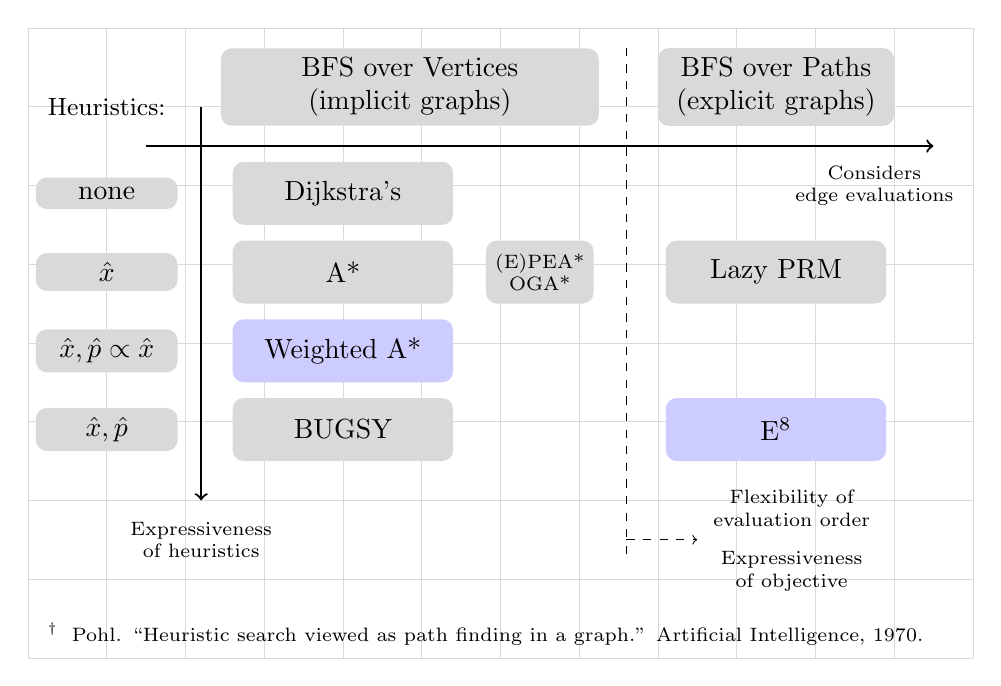
\begin{tikzpicture}
      \draw[step=1,black!15,very thin,opacity=\gridopacity] (0,0) grid (12,8);
      
      \node[align=center,fill=black!15,minimum width=4.8cm,rounded corners]
         at (4.85,7.25) {BFS over Vertices\\(implicit graphs)};
      \node[align=center,fill=black!15,minimum width=3cm,rounded corners]
         at (9.5,7.25) {BFS over Paths\\(explicit graphs)};
      
      \draw[dashed] (7.6,7.75) -- (7.6,1.25);
      \draw[dashed,->] (7.6,1.5) -- (8.5,1.5);
      \node[align=center,font=\scriptsize]
         at (9.7,1.9) {Flexibility of\\evaluation order};
      \node[align=center,font=\scriptsize]
         at (9.7,1.1) {Expressiveness\\of objective};

      % x axis
      \draw[->,thick] (1.5,6.5) -- (11.5,6.5);
      \node[align=center,font=\scriptsize]
         at (10.75,6) {Considers\\edge evaluations};
      
      \node[font=\small] at (1,7) {Heuristics:};
      
      % y axis
      \draw[->,thick] (2.2,7) -- (2.2,2);
      \node[align=center,font=\scriptsize]
         at (2.2,1.5) {Expressiveness\\of heuristics};

      \node[align=center,fill=black!15,rounded corners,minimum width=1.8cm,minimum height=0.4cm]
         at (1,5.9) {none};
      \node[fill=black!15,rounded corners,minimum height=0.8cm,minimum width=2.8cm]
         at (4,5.9) {Dijkstra's};

      \node[align=center,fill=black!15,rounded corners,minimum width=1.8cm,minimum height=0.4cm]
         at (1,4.9) {${\hat x}$};
      \node[fill=black!15,rounded corners,minimum height=0.8cm,minimum width=2.8cm]
         at (4,4.9) {A*};
      \node[fill=black!15,rounded corners,minimum height=0.8cm,font=\scriptsize,align=center]
         at (6.5,4.9) {(E)PEA*\\OGA*};
      \node[fill=black!15,rounded corners,minimum height=0.8cm,minimum width=2.8cm]
         at (9.5,4.9) {Lazy PRM};
      
      \only<2>{
         \node[align=center,fill=black!15,rounded corners,minimum width=1.8cm,minimum height=0.4cm]
            at (1,3.9) {${\hat x}, {\hat p} \propto {\hat x}$};
         \node[fill=blue!20,rounded corners,minimum height=0.8cm,minimum width=2.8cm]
            at (4,3.9) {Weighted A*};
      }
      
      \node[align=center,fill=black!15,rounded corners,minimum width=1.8cm,minimum height=0.4cm]
         at (1,2.9) {${\hat x}, {\hat p}$};
      \node[fill=black!15,rounded corners,minimum height=0.8cm,minimum width=2.8cm]
         at (4,2.9) {BUGSY};
      \node[fill=blue!20,rounded corners,minimum height=0.8cm,minimum width=2.8cm]
         at (9.5,2.9) {E$^8$};
      
      \only<2>{
         \node at (6,0.3) {\begin{minipage}{11.5cm}\scriptsize{
            $^\dag$\PaperPortrait\; Pohl. ``Heuristic search viewed as path finding in a graph.''
            Artificial Intelligence, 1970.
         }\end{minipage}};
      }
      
   \end{tikzpicture}
\end{frame}

\begin{frame}
   \frametitle{Example Problem}
   \begin{tikzpicture}
   
      \draw[step=1,black!15,very thin,opacity=\gridopacity] (0,0) grid (12,8);
      
      \node[inner sep=0pt] at (6,4.75) {%
         \only<1>{\includegraphics[width=5cm]{build/e8-world-intro}}%
         \only<2>{\includegraphics[width=5cm]{build/e8-world-astar}}%
         \only<3>{\includegraphics[width=5cm]{build/e8-world-wastar}}%
         \only<4>{\includegraphics[width=5cm]{build/e8-world-e8}}%
      };
      
      \node[inner sep=0pt] at (6,1) {\begin{minipage}{6cm}\centering%
         \only<2>{
            A*\\
            Planning Effort: 692.3 \\%\worldstatsastarplan\\
            Execution Effort: 14.2 \\%\worldstatsastarexec\\
            Total Effort: 706.5
         }
         \only<3>{
            Weighted A* ($\epsilon=3$)\\
            Planning Effort: 390.8 \\%\worldstatswastarplan\\
            Execution Effort: 18.5 \\%\worldstatswastarexec\\
            Total Effort: 409.3
         }
         \only<4>{
            E$^8$ ($\lambda=0.5$)\\
            Planning Effort: 358.8 \\%\worldstatseEplan\\
            Execution Effort: 20.5 \\%\worldstatseEexec\\
            Total Effort: 379.3
         }
      \end{minipage}};
      
   \end{tikzpicture}
\end{frame}

%\begin{frame}
%   \frametitle{Multiple Queries}
%   \begin{tikzpicture}
%      \draw[step=1,black!15,very thin,opacity=\gridopacity] (0,0) grid (12,8);
%      
%      \node[inner sep=0pt] at (6,7.4) {\begin{minipage}{12cm}\centering
%         Implicit algorithms manifest planning effort in
%         {\bf computed g-values}.
%         Explicit algorithms manifest planning effort in
%         {\bf evaluated edges}.
%      \end{minipage}};
%      
%      \begin{scope}[shift={(0,0.8)}]
%         \clip (0,4.5) rectangle (12,6);
%         \node[fill=blue!20,rounded corners,minimum height=5.8cm,minimum width=8.4cm] at (6,3) {};
%         \node[inner sep=0,anchor=north] at (6,5.8) {\begin{minipage}{8cm}\small{
%         \begin{algorithmic}[1]
%            \Procedure {E$^8$}{$G,
%               V_{\mbox{\scriptsize start}}, V_{\mbox{\scriptsize goal}},
%               \mathcal{M}, \lambda$}
%            \State $x_{\mbox{\scriptsize eval}}[\cdot] \leftarrow$ empty map
%               ($E \rightarrow \mathbb{R}_0^+$)
%            \State $\dots$
%            \EndProcedure
%         \end{algorithmic}
%         }\end{minipage}};
%      \end{scope}
%      
%      \node[inner sep=0] at (3,2.6) {
%         \includegraphics{build/talk-act1-2d,astars}
%      };
%      \node[inner sep=0] at (9,2.6) {
%         \includegraphics{build/talk-act1-2d,astars}
%      };
%   
%   \end{tikzpicture}
%\end{frame}

\begin{frame}
   \frametitle{Survey of Graph Search Algorithms}
   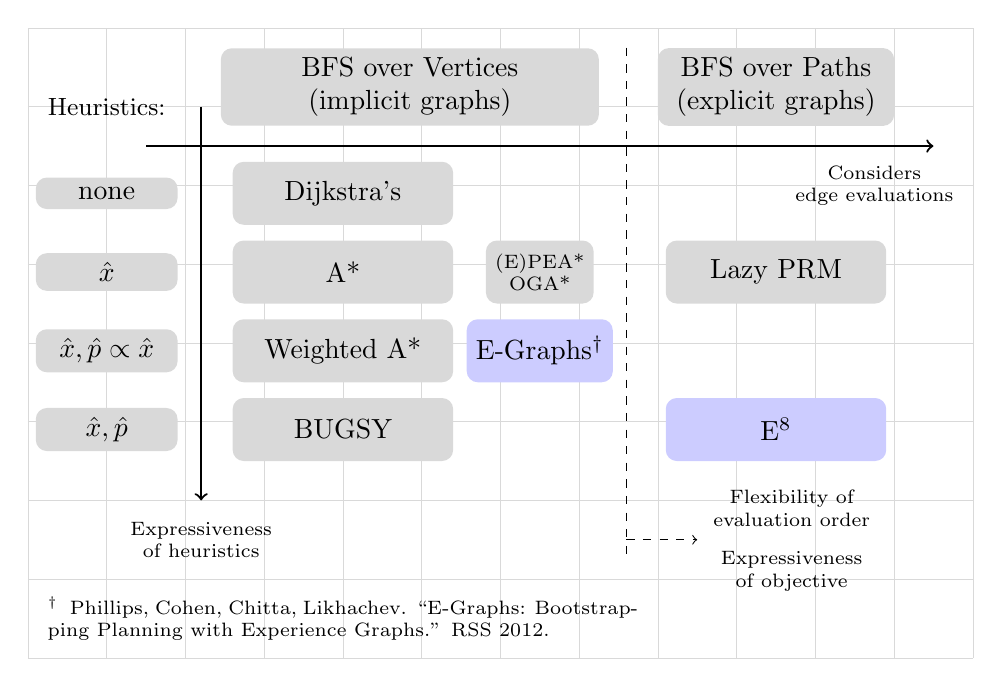
\begin{tikzpicture}
      \draw[step=1,black!15,very thin,opacity=\gridopacity] (0,0) grid (12,8);
      
      \node[align=center,fill=black!15,minimum width=4.8cm,rounded corners]
         at (4.85,7.25) {BFS over Vertices\\(implicit graphs)};
      \node[align=center,fill=black!15,minimum width=3cm,rounded corners]
         at (9.5,7.25) {BFS over Paths\\(explicit graphs)};
      
      \draw[dashed] (7.6,7.75) -- (7.6,1.25);
      \draw[dashed,->] (7.6,1.5) -- (8.5,1.5);
      \node[align=center,font=\scriptsize]
         at (9.7,1.9) {Flexibility of\\evaluation order};
      \node[align=center,font=\scriptsize]
         at (9.7,1.1) {Expressiveness\\of objective};

      % x axis
      \draw[->,thick] (1.5,6.5) -- (11.5,6.5);
      \node[align=center,font=\scriptsize]
         at (10.75,6) {Considers\\edge evaluations};
      
      \node[font=\small] at (1,7) {Heuristics:};
      
      % y axis
      \draw[->,thick] (2.2,7) -- (2.2,2);
      \node[align=center,font=\scriptsize]
         at (2.2,1.5) {Expressiveness\\of heuristics};

      \node[align=center,fill=black!15,rounded corners,minimum width=1.8cm,minimum height=0.4cm]
         at (1,5.9) {none};
      \node[fill=black!15,rounded corners,minimum height=0.8cm,minimum width=2.8cm]
         at (4,5.9) {Dijkstra's};

      \node[align=center,fill=black!15,rounded corners,minimum width=1.8cm,minimum height=0.4cm]
         at (1,4.9) {${\hat x}$};
      \node[fill=black!15,rounded corners,minimum height=0.8cm,minimum width=2.8cm]
         at (4,4.9) {A*};
      \node[fill=black!15,rounded corners,minimum height=0.8cm,font=\scriptsize,align=center]
         at (6.5,4.9) {(E)PEA*\\OGA*};
      \node[fill=black!15,rounded corners,minimum height=0.8cm,minimum width=2.8cm]
         at (9.5,4.9) {Lazy PRM};
      
      \node[align=center,fill=black!15,rounded corners,minimum width=1.8cm,minimum height=0.4cm]
         at (1,3.9) {${\hat x}, {\hat p} \propto {\hat x}$};
      \node[fill=black!15,rounded corners,minimum height=0.8cm,minimum width=2.8cm]
         at (4,3.9) {Weighted A*};
      \only<2>{
         \node[fill=blue!20,rounded corners,minimum height=0.8cm]
            at (6.5,3.9) {E-Graphs$^\dag$};
      }
      
      \node[align=center,fill=black!15,rounded corners,minimum width=1.8cm,minimum height=0.4cm]
         at (1,2.9) {${\hat x}, {\hat p}$};
      \node[fill=black!15,rounded corners,minimum height=0.8cm,minimum width=2.8cm]
         at (4,2.9) {BUGSY};
      \node[fill=blue!20,rounded corners,minimum height=0.8cm,minimum width=2.8cm]
         at (9.5,2.9) {E$^8$};
      
      %\only<2>{
      %   \node at (6,0.3) {\begin{minipage}{11.5cm}\scriptsize{
      %      $^\dag$\PaperPortrait\; Pohl. ``Heuristic search viewed as path finding in a graph.''
      %      Artificial Intelligence, 1970.
      %   }\end{minipage}};
      %}

      \only<2>{
         \node at (4,0.5) {\begin{minipage}{7.5cm}\scriptsize{
            $^\dag$\PaperPortrait\; Phillips, Cohen, Chitta, Likhachev.
            ``E-Graphs: Bootstrapping Planning with Experience Graphs.''
            RSS 2012.
         }\end{minipage}};
      }
      
   \end{tikzpicture}
\end{frame}

\begin{frame}
   \frametitle{Multiple Queries: Relationship to Experience Graphs}
   \begin{tikzpicture}
      \draw[step=1,black!15,very thin,opacity=\gridopacity] (0,0) grid (12,8);
      
      \node[anchor=north,fill=blue!20,rounded corners] at (6,7.75) {\begin{minipage}{9cm}\small{
         E$^8$ objective with ${\hat p}(e) = \alpha {\hat x}(e)$ and $\lambda < 1$:
         \begin{equation*}
            \arraycolsep=1.4pt
            \hat{f}(\pi) \propto \sum_{e \in \pi} \left\{
            \begin{array}{cl}
               x(e) & \mbox{if edge } e \mbox{ evaluated} \\
               \left[ 1 + \frac{\alpha \lambda}{1-\lambda} \right] \hat{x}(e) & \mbox{otherwise} \\
            \end{array}
            \right.
         \end{equation*}
      }\end{minipage}};
      
      \only<2->{
         \node[anchor=north,fill=black!15,rounded corners] at (6,5.5) {\begin{minipage}{10cm}\small{
            Experience Graphs$^\dag$ objective, expressed explicitly over paths:
            \begin{equation*}
               \arraycolsep=1.4pt
               \hat{f}_{\ms{EG}}(\pi) \propto \sum_{e \in \pi} \left\{
               \begin{array}{cl}
                  x(e) & \mbox{if edge } e \mbox{ evaluated, this search} \\
                  \epsilon \, x(e) & \mbox{if edge } e \mbox{ evaluated, previous solution} \\
                  \epsilon \, \epsilon^E \, \hat{x}(e) & \mbox{otherwise} \\
               \end{array}
               \right.
            \end{equation*}
         }\end{minipage}};
      }
      
      \only<3->{
         \node[anchor=north] at (6,2.75) {\begin{minipage}{11.5cm}\small{
            E$^8$ and E-Graphs are equivalent under the following
            conditions:
            \begin{itemize}
            \item ${\hat p}(e) = \alpha \, {\hat x}(e)$
            \item $\epsilon^E = 1 + \frac{\alpha \lambda}{1-\lambda},
               \epsilon = 1, \lambda < 1$
            \item Only edges from the solution path are kept between queries
            \end{itemize}
         }\end{minipage}};
      }
      
      \only<1-2>{
         \node at (4,0.5) {\begin{minipage}{7.5cm}\scriptsize{
            $^\dag$\PaperPortrait\; Phillips, Cohen, Chitta, Likhachev.
            ``E-Graphs: Bootstrapping Planning with Experience Graphs.''
            RSS 2012.
         }\end{minipage}};
      }
      
   \end{tikzpicture}
\end{frame}

\begin{frame}
   \frametitle{E$^8$ Search Summary}
   \begin{tikzpicture}

      \draw[step=1,black!15,very thin,opacity=\gridopacity] (0,0) grid (12,8);

      \node[anchor=south,shape=document,draw,inner sep=0.25cm]
      at (4,4.5) {\begin{minipage}{5cm}\small{
         Ensemble Effort model $\mathcal{M}$: \\
         $x(e)$ : edge evaluation function \\
         ${\hat x}(e)$ : execution effort estimate \\
         ${\hat p}(e)$ : planning effort estimate
      }\end{minipage}};
      
      \node[anchor=south,shape=document,draw,align=center]
      at (9,4.5) {
         Graph G:\\
         \includegraphics[width=2.5cm]{build/roadmap-2d-simple}
         %\includegraphics[width=2.5cm]{build/talk-act1-2d,graph}
         
      };
      
      \draw[->,line width=1pt] (6.3,4.4) -- (6.3,3.9);
      \draw[->,line width=1pt] (7.8,4.4) -- (7.8,3.9);
      
      \node[fill=blue!20,minimum height=1.5cm,minimum width=2.5cm,
         align=center,rounded corners,inner ysep=0.7cm]
      at (7,2.5) {
         E$^8$ Search\\
         \small{$\min
         \left[ (1 - \lambda) \hat{f}_x + \lambda \hat{f}_p \right]$}
      };
      
      \node[shape=document,draw,align=center,inner xsep=10pt]
      at (2.4,3) {
         Query $V_{s1}$, $V_{g1}$, $\lambda_1$
      };
      \draw[->,line width=1pt] (4.5,3) -- (5.0,3);
      
      \draw[->,line width=1pt] (9,3) -- (9.5,3);
      \node[shape=document,draw,align=center,inner xsep=5pt]
      at (10.1,3) {$\pi^*_1$\;\;};
      
      \node[shape=document,draw,align=center,inner xsep=10pt]
      at (2.4,2) {
         Query $V_{s2}$, $V_{g2}$, $\lambda_2$
      };
      \draw[->,line width=1pt] (4.5,2) -- (5.0,2);
      
      \draw[->,line width=1pt] (9,2) -- (9.5,2);
      \node[shape=document,draw,align=center,inner xsep=5pt]
      at (10.1,2) {$\pi^*_2$\;\;};

   \end{tikzpicture}
\end{frame}

\begin{frame}
   \frametitle{The Planning vs. Execution Tradeoff on Roadmaps}
   \begin{tikzpicture}
      \draw[step=1,black!15,very thin,opacity=\gridopacity] (0,0) grid (12,8);
      
      \node[inner sep=0] at (9,5) {%
         %{\only<1>{\includegraphics{build/talk-act1-2d,rootsonly}}}%
         %{\only<1-2>{\includegraphics{build/talk-act1-2d,cfree}}}%
         %{\only<3>{\includegraphics{build/talk-act1-2d,paths}}}%
         %{\only<3>{\includegraphics{build/talk-act1-2d,graph}}}%
         {\only<1->{\includegraphics{build/talk-act1-2d,astara}}}%
      };
      
      \node[draw,circle,inner sep=2pt,ultra thick,fill=red!50] at (7.05, 2.0) {};
      \node[draw,circle,inner sep=2pt,ultra thick,fill=green!50] at (7.5, 2.0) {};
      \node[anchor=west] at (7.9,2.0) {start, goal configs};
      \node[anchor=west,draw,line width=1pt,fill=blue!20,minimum width=0.75cm,minimum height=0.10cm]
         (Cfreebox) at (6.9, 1.5) {};
      \node[anchor=west] at (7.9,1.5) {$\mathcal{C}_{\mbox{\scriptsize free}}$};
      
      \node[anchor=north,fill=black!15,rounded corners] at (3,7.5)
      {\bf Focus: Roadmap methods};
      
      \only<2>{
         \node[anchor=north,fill=blue!20,rounded corners] at (3,6.5)
         {\begin{minipage}{5.5cm}
         1. Searching roadmap graphs
         
         - survey of search methods
         
         - propose new algorithm E$^8$
         \end{minipage}};
      }
      \only<1>{
         \node[anchor=north,fill=green!20,rounded corners] at (3,6.5)
         {\begin{minipage}{5.5cm}
         1. Searching roadmap graphs
         
         - survey of search methods
         
         - propose new algorithm E$^8$
         \end{minipage}};
      }
      
      \only<1>{
         \node[anchor=north,fill=blue!20,rounded corners] at (3,4.5)
         {\begin{minipage}{5.5cm}
         2. Research questions
         
         - graphs in C-space
         \end{minipage}};
      }
      \only<2>{
         \node[anchor=north,fill=green!20,rounded corners] at (3,4.5)
         {\begin{minipage}{5.5cm}
         2. Research questions
         
         - graphs in C-space
         \end{minipage}};
      }
   
   \end{tikzpicture}
\end{frame}

\begin{frame}
   \frametitle{E$^8$ Implementation}
   \begin{tikzpicture}
      \draw[step=1,black!15,very thin,opacity=\gridopacity] (0,0) grid (12,8);
   
      % alg
      \node[anchor=west,inner xsep=0pt,fill=black!15,minimum height=1.8cm,rounded corners]
      at (0,6.85) {\begin{minipage}{3.25cm}\small{
         \algrenewcommand\algorithmicindent{0.0cm}%
         \algrenewcommand\algorithmicloop{\!\!\!\!\textbf{loop}}
         \begin{algorithmic}
         \Loop%
            \State $\pi^* \leftarrow \argmin\limits_{\pi \in \Pi} \hat{f}(\pi)$
            \State \textsc{EvalPath}$(\pi^*)$
         \EndLoop
         \end{algorithmic}
      }\end{minipage}};
      
      % f(pi) execution path cost
      \node[anchor=west,inner xsep=0pt,fill=black!15,minimum height=1.8cm,rounded corners]
      at (3.5,6.85) {\begin{minipage}{8.5cm}\small{%
         \vspace{-0.3cm}
         \begin{equation*}%
            \arraycolsep=1.4pt
            \hat{f}(\pi) = \sum_{e \in \pi} \left\{
            \begin{array}{cl}
               (1-\lambda) x(e) & \mbox{if edge } e \mbox{ evaluated} \\
               (1-\lambda) \hat{x}(e) + \lambda \hat{p}(e) & \mbox{otherwise} \\
            \end{array}
            \right.
         \end{equation*}
      }\end{minipage}};
      
      % procedure background
      \only<2->{
         \node[fill=blue!20,rounded corners,minimum height=5.1cm,minimum width=11.4cm]
         at (6,3.2) {};
      }
      
      % procedure background highlights
      \only<3->{\fill[red!30] (0.3,1.175) rectangle (11.7,1.675);}
      \only<4->{\fill[green!30] (0.3,2.90) rectangle (11.7,3.40);}
      
      % procedure itself
      \only<2->{
         \node[inner sep=0] at (6,3.2) {\begin{minipage}{11cm}\small{
         \begin{algorithmic}[1]
            \Procedure {E$^8$}{$G,
               V_{\mbox{\scriptsize start}}, V_{\mbox{\scriptsize goal}},
               \mathcal{M}, \lambda$}
            \State $x_{\mbox{\scriptsize eval}}[\cdot] \leftarrow$ empty map
               ($E \rightarrow \mathbb{R}_0^+$)
            \ForAll {$e \in G$}
               \State $e.{\mbox{cost}} \leftarrow
                  (1 - \lambda) \, \hat{x}(e) + \lambda \, \hat{p}(e)$
                  \Comment Ensemble effort model
            \EndFor
            \Loop
               \State $\pi^* = \mbox{\sc BiDijkstras}(G,
                  V_{\mbox{\scriptsize start}}, V_{\mbox{\scriptsize goal}})$
               \State $e \leftarrow \mbox{select from } \pi
                  \;|\; e \notin x_{\mbox{\scriptsize eval}}$
               \If {$e = \mbox{\bf nil}$}
                  \State \Return $\pi^*$
               \EndIf
               \State $x_{\mbox{\scriptsize eval}}[e] \leftarrow x(e)$
                  \Comment Evaluate edge (expensive!)
               \State $e.{\mbox{cost}} \leftarrow
                  (1 - \lambda) \, x_{\mbox{\scriptsize eval}}[e]$
                  \Comment Update ensemble estimate
            \EndLoop
            \EndProcedure
         \end{algorithmic}
         }\end{minipage}};
      }
      
   \end{tikzpicture}
\end{frame}

\begin{frame}
   \frametitle{Continuous Spaces: E$^8$-PRM}
   \begin{tikzpicture}
      \draw[step=1,black!15,very thin,opacity=\gridopacity] (0,0) grid (12,8);
      
      \node[inner sep=0pt] at (6,7.4) {\begin{minipage}{11.5cm}\centering
         The E$^8$-PRM is agnostic to the type of roadmap used.
      \end{minipage}};
      
      \node[inner sep=0] at (4,5.5) {%
         \includegraphics[height=2.5cm]{build/roadmap-2d-densified}
      };
      
      \node[inner sep=0] at (8,5.5) {%
         \includegraphics[height=2.5cm]{figs/halton.png}
      };
      
      % procedure itself
      \node[fill=blue!20,rounded corners] at (6,2) {\begin{minipage}{11cm}\small{
         \begin{algorithmic}[1]
         \State $G \leftarrow \mbox{empty graph}$
         \State $\mathcal{M} \leftarrow
            \mathcal{M}_{\ms{dist}}
            + \mathcal{M}_{\ms{valid}}(\mathcal{C}_{\ms{free}})$
         \Procedure {E$^8$-PRM}{$G,
            V_{\mbox{\scriptsize start}}, V_{\mbox{\scriptsize goal}},
            N, \mathcal{M}, \lambda$}
         \State \textsc{AddRoots}($G, V_{\mbox{\scriptsize start}}, V_{\mbox{\scriptsize goal}}$)
         \Loop
            \State \textsc{PRMAddSamples}($G, \mathcal{C}, N$)
            \State $\pi^* \leftarrow \mbox{E}^8(G,
               V_{\mbox{\scriptsize start}}, V_{\mbox{\scriptsize goal}},
               \mathcal{M}, \lambda)$
            \If {$\mathcal{M}.\hat{x}(\pi^*) < \infty$}
               \State \Return $\pi^*$
            \EndIf
         \EndLoop
         \EndProcedure
         \end{algorithmic}
      }\end{minipage}};
      
   \end{tikzpicture}
\end{frame}

\begin{frame}
   \frametitle{Behavior of the E$^8$-PRM: Solution Paths}
   \begin{tikzpicture}
      \draw[step=1,black!15,very thin,opacity=\gridopacity] (0,0) grid (12,8);
   
      \node[draw,color=black!25,inner sep=1pt] (lambda0) at (3,6) {
         \includegraphics[width=5cm]{figs/bean-allpaths-lambda0.png}
      };
      \node[font=\small,below left=0cm of lambda0.north east] {$\lambda = 0$};
      
      \node[draw,color=black!25,inner sep=1pt] (lambda1) at (3,2) {
         \includegraphics[width=5cm]{figs/bean-allpaths-lambda1.png}
      };
      \node[font=\small,below left=0cm of lambda1.north east] {$\lambda = 1$};
      
      \begin{scope}[shift={(7.5,2.5)},font=\small]
      \begin{axis}[
         xlabel=Collision Checks,
         ylabel=Path Length,
         ylabel near ticks,
         xlabel near ticks,
         scaled x ticks=base 10:-3,
         scaled y ticks=base 10:-2,
         every x tick scale label/.style={
            at={(1,-0.2075)}
         },
         %ticks=none,
         axis lines=left,
         xmin=0,xmax=8000,
         ymin=700,ymax=950,
         width=5.5cm, height=5.5cm]
      
      \addplot[mark=*] plot coordinates { (7219.5, 733.0) };
      \addplot[mark=*] plot coordinates { (4692.6, 836.5) };
      \coordinate (l0) at (axis cs:7219.5, 733.0);
      \coordinate (l1) at (axis cs:4692.6, 836.5);
      
      \node (labl0) at ($ (l0) + (-250,15) $) {$\lambda=0$};
      \node (labl1) at ($ (l1) + (-250,15) $) {$\lambda=1$};
      \draw[->] (labl0) -- ($ (l0)!0.25cm!(labl0) $);
      \draw[->] (labl1) -- ($ (l1)!0.25cm!(labl1) $);

      \end{axis}
      \end{scope}
   
   \end{tikzpicture}
\end{frame}

\begin{frame}
   \frametitle{E$^8$ Implementation}
   \begin{tikzpicture}
      \draw[step=1,black!15,very thin,opacity=\gridopacity] (0,0) grid (12,8);
   
      \only<1>{
         % alg
         \node[anchor=west,inner xsep=0pt,fill=black!15,minimum height=1.8cm,rounded corners]
         at (0,6.85) {\begin{minipage}{3.25cm}\small{
            \algrenewcommand\algorithmicindent{0.0cm}%
            \algrenewcommand\algorithmicloop{\!\!\!\!\textbf{loop}}
            \begin{algorithmic}
            \Loop%
               \State $\pi^* \leftarrow \argmin\limits_{\pi \in \Pi} \hat{f}(\pi)$
               \State \textsc{EvalPath}$(\pi^*)$
            \EndLoop
            \end{algorithmic}
         }\end{minipage}};
         
         % f(pi) execution path cost
         \node[anchor=west,inner xsep=0pt,fill=black!15,minimum height=1.8cm,rounded corners]
         at (3.5,6.85) {\begin{minipage}{8.5cm}\small{%
            \vspace{-0.3cm}
            \begin{equation*}%
               \arraycolsep=1.4pt
               \hat{f}(\pi) = \sum_{e \in \pi} \left\{
               \begin{array}{cl}
                  (1-\lambda) x(e) & \mbox{if edge } e \mbox{ evaluated} \\
                  (1-\lambda) \hat{x}(e) + \lambda \hat{p}(e) & \mbox{otherwise} \\
               \end{array}
               \right.
            \end{equation*}
         }\end{minipage}};
      }
      
      % research question
      \only<2>{
         \node[fill=blue!20,rounded corners] at (6,6.85) {\begin{minipage}{9cm}
            {\bf Research Question Q1:}\\
            How can incremental graph search (e.g. LPA*$^\dag$)
            \\be used to efficiently implement the E$^8$ algorithm?
         \end{minipage}};
      }
      
      % procedure background
      \node[fill=blue!20,rounded corners,minimum height=5.1cm,minimum width=11.4cm]
      at (6,3.2) {};
      
      % procedure background highlights
      \fill[red!30] (0.3,1.175) rectangle (11.7,1.675);
      \fill[green!30] (0.3,2.90) rectangle (11.7,3.40);
      
      % procedure itself
      \node[inner sep=0] at (6,3.2) {\begin{minipage}{11cm}\small{
      \begin{algorithmic}[1]
         \Procedure {E$^8$}{$G,
            V_{\mbox{\scriptsize start}}, V_{\mbox{\scriptsize goal}},
            \mathcal{M}, \lambda$}
         \State $x_{\mbox{\scriptsize eval}}[\cdot] \leftarrow$ empty map
            ($E \rightarrow \mathbb{R}_0^+$)
         \ForAll {$e \in G$}
            \State $e.{\mbox{cost}} \leftarrow
               (1 - \lambda) \, \hat{x}(e) + \lambda \, \hat{p}(e)$
               \Comment Ensemble effort model
         \EndFor
         \Loop
            \State $\pi^* = \mbox{\sc BiDijkstras}(G,
               V_{\mbox{\scriptsize start}}, V_{\mbox{\scriptsize goal}})$
            \State $e \leftarrow \mbox{select from } \pi
               \;|\; e \notin x_{\mbox{\scriptsize eval}}$
            \If {$e = \mbox{\bf nil}$}
               \State \Return $\pi^*$
            \EndIf
            \State $x_{\mbox{\scriptsize eval}}[e] \leftarrow x(e)$
               \Comment Evaluate edge (expensive!)
            \State $e.{\mbox{cost}} \leftarrow
               (1 - \lambda) \, x_{\mbox{\scriptsize eval}}[e]$
               \Comment Update ensemble estimate
         \EndLoop
         \EndProcedure
      \end{algorithmic}
      }\end{minipage}};
      
      \only<2>{
         \node at (6,0.3) {\begin{minipage}{11.5cm}\scriptsize{
            $^\dag$\PaperPortrait\; Koenig, Likhachev, Furcy.
            ``Lifelong Planning A*.''
            Artificial Intelligence Journal, 2004.
         }\end{minipage}};
      }
      
   \end{tikzpicture}
\end{frame}

\begin{frame}
   \frametitle{The Planning vs. Execution Tradeoff on Roadmaps}
   \begin{tikzpicture}
      \draw[step=1,black!15,very thin,opacity=\gridopacity] (0,0) grid (12,8);
      
      \node[inner sep=0] at (9,5) {
         \includegraphics{build/talk-act1-2d,graph}
      };
      
      \node[draw,circle,inner sep=2pt,ultra thick,fill=red!50] at (7.05, 2.0) {};
      \node[draw,circle,inner sep=2pt,ultra thick,fill=green!50] at (7.5, 2.0) {};
      \node[anchor=west] at (7.9,2.0) {start, goal configs};
      \node[anchor=west,draw,line width=1pt,fill=blue!20,minimum width=0.75cm,minimum height=0.10cm]
         (Cfreebox) at (6.9, 1.5) {};
      \node[anchor=west] at (7.9,1.5) {$\mathcal{C}_{\mbox{\scriptsize free}}$};
      
      \node[anchor=north,fill=black!15,rounded corners] at (3,7.5)
      {\bf Focus: Roadmap methods};
      
      \node[anchor=north,fill=blue!20,rounded corners] at (3,6.5)
      {\begin{minipage}{5.5cm}
      1. Searching roadmap graphs
      
      - survey of search methods
      
      - propose new algorithm E$^8$
      \end{minipage}};
      
      \only<1>{
         \node[anchor=north,fill=green!20,rounded corners] at (3,4.5)
         {\begin{minipage}{5.5cm}
         2. Research questions
         
         - graphs in C-space
         \end{minipage}};
      }
      \only<2>{
         \node[anchor=north,fill=blue!20,rounded corners] at (3,4.5)
         {\begin{minipage}{5.5cm}
         2. Research questions
         
         - graphs in C-space
         \end{minipage}};
         
         \node[anchor=north,fill=black!15,rounded corners] at (3,3.0)
            {Comparison to RRT?};
      }
      
   \end{tikzpicture}
\end{frame}

\begin{frame}
   \frametitle{Behavior of the E$^8$-PRM: Maze RRT Comparison}
   \begin{tikzpicture}
      \draw[step=1,black!15,very thin,opacity=\gridopacity] (0,0) grid (12,8);
      
      % e8 prm on left side top
      \fill[blue!50] (0.1,2.8) rectangle (2.7,7.9);
      \node[inner sep=0pt] (lambda0) at (1.4,6.6) {
         \includegraphics[width=2.5cm]{figs/compare-2d-rrtc1-checkmask-l00-s1.png}
      };
      \node[font=\scriptsize,below left=0cm of lambda0.north east] {$\lambda = 0$};
      \node[inner sep=0pt] (lambda1) at (1.4,4.1) {
         \includegraphics[width=2.5cm]{figs/compare-2d-rrtc1-checkmask-l10-s1.png}
      };
      \node[font=\scriptsize,below left=0cm of lambda1.north east] {$\lambda = 1$};
      
      % rrts along bottom
      \fill[red!50] (1.15,0.1) rectangle (6.4,2.7);
      \node[inner sep=0pt] (conconr1) at (2.5,1.4) {
         \includegraphics[width=2.5cm]{figs/compare-2d-rrtc1-rrtconcon-r1-s1.png}
      };
      \node[font=\scriptsize,below left=0cm of conconr1.north east] {$R = 1$};
      \node[inner sep=0pt] (conconr6) at (5.05,1.4) {
         \includegraphics[width=2.5cm]{figs/compare-2d-rrtc1-rrtconcon-r6-s1.png}
      };
      \node[font=\scriptsize,below left=0cm of conconr6.north east] {$R = 6$};
      \fill[green!50] (6.65,0.1) rectangle (11.9,2.7);
      \node[inner sep=0pt] (extconr1) at (8.0,1.4) {
         \includegraphics[width=2.5cm]{figs/compare-2d-rrtc1-rrtextcon-r1-s1.png}
      };
      \node[font=\scriptsize,below left=0cm of extconr1.north east] {$R = 1$};
      \node[inner sep=0pt] (extconr6) at (10.55,1.4) {
         \includegraphics[width=2.5cm]{figs/compare-2d-rrtc1-rrtextcon-r6-s1.png}
      };
      \node[font=\scriptsize,below left=0cm of extconr6.north east] {$R = 6$};

      % plot
      \node[inner sep=0pt] at (7.5,5.9) {
         \includegraphics[width=9cm]{build/maze-plot-ensemble}
      };
      
      \node at (8.5,3.1) {\begin{minipage}{6.5cm}\scriptsize{
         \PaperPortrait\; Kuffner, LaValle.
         ``RRT-connect: An efficient approach to single-query path planning.''
         ICRA 2000.
      }\end{minipage}};
      
   \end{tikzpicture}
\end{frame}

\begin{frame}
   \frametitle{HERB Example Problem}
   \begin{tikzpicture}
      \draw[step=1,black!15,very thin,opacity=\gridopacity] (0,0) grid (12,8);
   
      \node[inner sep=0pt]
         at ( 1.50,6.5) {\includegraphics[width=2cm]{figs/testherb-a.png}};
      \node[inner sep=0pt]
         at ( 3.75,6.5) {\includegraphics[width=2cm]{figs/testherb-b.png}};
      \node[inner sep=0pt]
         at ( 6.00,6.5) {\includegraphics[width=2cm]{figs/testherb-c.png}};
      \node[inner sep=0pt]
         at ( 8.25,6.5) {\includegraphics[width=2cm]{figs/testherb-d.png}};
      \node[inner sep=0pt]
         at (10.50,6.5) {\includegraphics[width=2cm]{figs/testherb-e.png}};

      \node[inner sep=0pt]
         at ( 2,3) {\includegraphics[width=3.9cm]{build/herb-mugbin-plot-1-eprm}};
      \node[inner sep=0pt]
         at ( 6,3) {\includegraphics[width=3.9cm]{build/herb-mugbin-plot-2-eprm}};
      \node[inner sep=0pt]
         at ( 10,3) {\includegraphics[width=3.9cm]{build/herb-mugbin-plot-3-eprm}};
   
   \end{tikzpicture}
\end{frame}

\begin{frame}
   \frametitle{Experiments in 2D and 7D}
   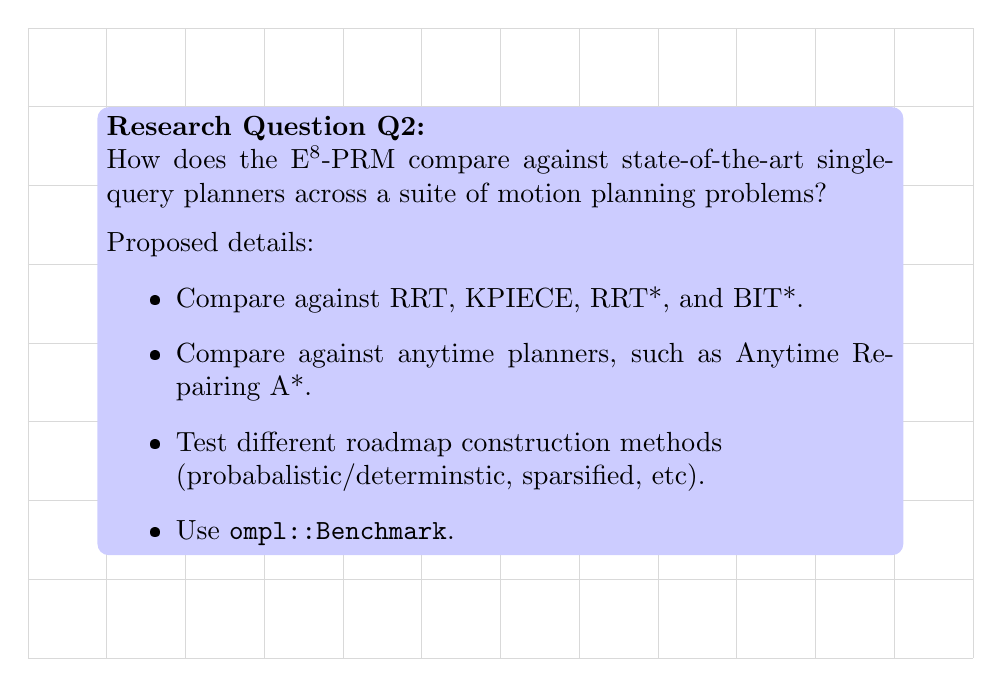
\begin{tikzpicture}
      \draw[step=1,black!15,very thin,opacity=\gridopacity] (0,0) grid (12,8);
   
      \node[anchor=north,fill=blue!20,rounded corners] at (6,7) {\begin{minipage}{10cm}
         {\bf Research Question Q2:}\\
         How does the E$^8$-PRM compare against state-of-the-art
         single-query planners across a suite of motion planning problems?
         
         \medskip
         Proposed details:
         \begin{itemize}
         \item Compare against RRT, KPIECE, RRT*, and BIT*.
         \item Compare against anytime planners, such as Anytime Repairing A*.
         \item Test different roadmap construction methods \\
            (probabalistic/determinstic, sparsified, etc).
         \item Use {\tt ompl::Benchmark}.
         \end{itemize}
      \end{minipage}};
   
   \end{tikzpicture}
\end{frame}

%\begin{frame}
%   \frametitle{E$^8$ Search and the E$^8$-PRM}
%   
%   This is a summary slide.
%   
%   $\lambda = 0$ : we only care about execution effort.  Lazy PRM.
%   
%   $\lambda = 1$ : we only care about planning effort.
%\end{frame}

\begin{frame}
   \frametitle{Part 1: Capturing the Planning/Execution Tradeoff}
      \begin{tikzpicture}
      \draw[step=1,black!15,very thin,opacity=\gridopacity] (0,0) grid (12,8);
   
      % figure adapted from proposal doc
      \begin{scope}[font=\scriptsize,shift={(1.5,6.25)}]
         
         % root sets
         \node[draw,black,rounded corners,minimum height=1.5cm,minimum width=1cm]
            (Xgrasp) at (3,0) {};
         \node[above=0cm of Xgrasp] {Grasp};
         \node[draw,black,rounded corners,minimum height=1.5cm,minimum width=1cm]
            (Xdrop) at (6,0) {};
         \node[above=0cm of Xdrop] {Place};
         
         % nodes
         \node[circle,fill=black,inner sep=2] (xstart) at (0,0) {};
         \node[above=0.1cm of xstart] {$q_{\mbox{\scriptsize start}}$};
         
         % grasp choices
         \node[circle,fill=black,inner sep=2] (xg1) at (2.8,0.5) {};
         \node[circle,fill=black,inner sep=2] (xg2) at (3.1,0.1) {};
         \node[circle,fill=black,inner sep=2] (xg3) at (2.9,-0.5) {};
         % place choices
         \node[circle,fill=black,inner sep=2] (xd1) at (5.9,0.3) {};
         \node[circle,fill=black,inner sep=2] (xd2) at (6.0,-0.4) {};
         % xend 
         \node[circle,fill=black,inner sep=2] (xend) at (9,0) {};
         \node[above=0.1cm of xend] {$q_{\mbox{\scriptsize end}}$};
         
         \draw[line width=1.5mm,white]
            (xstart) .. controls (1,0.2) and (1.4,0.9) .. (xg1);
         \draw[line width=1.5mm,white]
            (xstart) .. controls (1.5,0.2) .. (xg2);
         \draw[line width=1.5mm,white]
            (xstart) .. controls (1.8,-0.6) and (1.6,-0.8) .. (xg3);
         \draw
            (xstart) .. controls (1,0.2) and (1.4,0.9) .. (xg1);
         \draw
            (xstart) .. controls (1.5,0.2) .. (xg2);
         \draw
            (xstart) .. controls (1.8,-0.6) and (1.6,-0.8) .. (xg3);
         \draw[line width=1.5mm,white]
            (xg1) -- (4.7,0.6);
         \draw
            (xg1) -- (4.7,0.6);
         \draw[line width=1.5mm,white]
            (xg2) .. controls (4.5,1) and (3.5,-1.2) .. (4.5,-0.4)
                  .. controls (5.5,0.5) and (5.0,-1.3) .. (xd2);
         \draw
            (xg2) .. controls (4.5,1) and (3.5,-1.2) .. (4.5,-0.4)
                  .. controls (5.5,0.5) and (5.0,-1.3) .. (xd2);
         \draw[line width=1.5mm,white]
            (xg3) .. controls (4.3, 0.2) and (4.5,-0.2) .. (xd1);
         \draw
            (xg3) .. controls (4.3, 0.2) and (4.5,-0.2) .. (xd1);
         % in s3
         \draw[line width=1.5mm,white]
            (xd1) .. controls (8,0.3) and (8,0.1) .. (xend);
         \draw
            (xd1) .. controls (8,0.3) and (8,0.1) .. (xend);
         
         \node[fill,black,rounded corners,minimum height=1.5cm,minimum width=1cm,
            opacity=0.1] at (3,0) {};
         \node[fill,black,rounded corners,minimum height=1.5cm,minimum width=1cm,
            opacity=0.1] at (6,0) {};
         
      \end{scope}
   
      \fill[green!20] (0.1,3.7) rectangle (11.9,4.3);
   
      \node[anchor=north] at (6,5) {\begin{minipage}{11.5cm}
         Planning for manipulation tasks poses three challenges:
         
         \begin{itemize}
         \item Challenge 1: Capturing the planning/execution tradeoff..
         \item Challenge 2: Incongruent steps impede reuse.
         \item Challenge 3: Coupled steps require long planning horizons.
         \end{itemize}
      \end{minipage}};
   
   \end{tikzpicture}
\end{frame}
